Bei fast allen Varianten des TF mit Kaskadennetzwerken kommt es nach TF zu einer Stabilisierung der Performanz des Netzes. 
Diese wird hier genauer vorgestellt und erklärt. 

\begin{figure}[htpb]
    \includegraphics[height=5cm]{../../Plots/ba_plots/convmaxpool/convmaxpooltrainbig.png}
    \includegraphics[height=5cm]{../../Plots/ba_plots/convmaxpool/convmaxpooltestbig.png}
    \caption{\label{fig:cmptrbig} Stabilisierung der Performanz}
\end{figure}

Es ist in Figure 3.4 links deutlich zu erkennen, dass es bereits nach zehn Epochen nach TF zu einer Stabilisierung der Accuracy kommt. 
Selbst bei späteren Epochen mit mehr Layern verbessert sich diese nur noch wenig. Dies bestätigt auch der Plot von den Testdaten, dessen 
Werte schlagartig nach TF besser wird, aber danach nur noch wenig steigen. 

Dasselbe verhält sich auch bei Regressionsnetzwerken. Nach TF kommt es schnell dazu, dass sich der Mean Absolute Error nicht weiter verringert. 
Ein Beispielplot ist in Figure 3.5 zu sehen. 

\begin{figure}[htpb]
    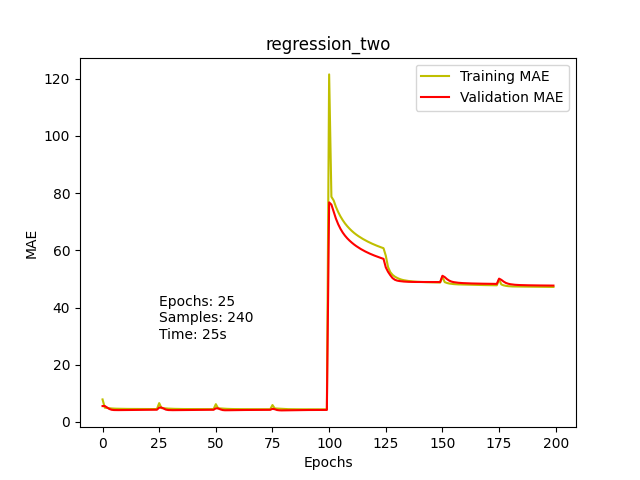
\includegraphics[height=5cm]{../../Plots/ba_plots/regr2/regr2train.png}
    \caption{\label{fig:regr2tr} Stabilisierung bei Regression}
\end{figure}

Diese Stabilisierung der Performanz ist sehr schnell nach TF. Dies fällt dann auf, wenn direkt auf dem Targetdatensatz gelernt wird. 
% Targetdatensatz only Plot -> Diesen auch für das nächste Unterkapitel nutzen. 

\begin{figure}[htpb]
    \includegraphics[height=5cm]{../../Plots/ba_plots/convmaxpool/woconvmaxpoolbig.png}
    \caption{\label{fig:cmpwotf} Ohne TF}
\end{figure}

Wie in Figure 3.6 zu sehen, ist diese Stabilisierung ohne TF nach gleich vielen Epochen bezüglich des Datensatzes und es bleibt auch bei diesem 
Wert. Dies liegt an der händisch definierten Learningrate, die die Deep Cascade Netze haben. Die Learningrate für Klassifikation ist hierbei: 

\begin{equation}
    (10^{-4} * 10)^{\frac{10}{epoch + 10}}
\end{equation}

Die zweite Learningrate ist für die Regressionsnetzwerke. 

\begin{equation}
    (10^{-4} * 100)^{\frac{10}{epoch + 10}}
\end{equation}

Beide Learningraten haben die Eigenschaft, dass sie immer kleiner werden, wodurch diese Stabilisierung kommt. 

% Hier irgendwo die Learningrate hinzufügen


